\chapter{State of Art}
\label{ch:State of Art}

\section{Ball Seat Valve}
\label{Ball Seat Valve}

Check valves are one of the most widely utilized piping components in industrial metal piping systems. 
According to the classification of kinetics, a check valve is an automatically operated valve that
relies on its own weight and the pressure of the medium itself to prevent the backflow 
of the medium.\cite{kineticsValve}\\

The metallic ball seat valve used in this study is a check valve, which restricts the flow of fluid to
only one particular direction. The principle of action is to rely on the weight of the ball itself and 
the pressure of the medium, such as fluid or gas, to produce a downward normal force on the ball 
so that the ball is tightly pressed against the seat to stop the flow of the medium and thus prevent 
the fluid from flowing in the other direction. These seat valves play an important 
role in hydraulic and pneumatic systems.\\


Only the most fundamental components of the ball seat valve that play a critical role in its sealing 
are going to be covered in this article. The ball seat valve, which is depicted in Fig.\Ref{fig:ballseatvalve}, is made 
up of a ball with a radius of 20 millimeters and a seat that has an inner radius 
of 7.5 millimeters and a slope angle of 45 degrees. Both of these components are made of stainless steel.\\

\begin{figure}[htbp]
    \centering
    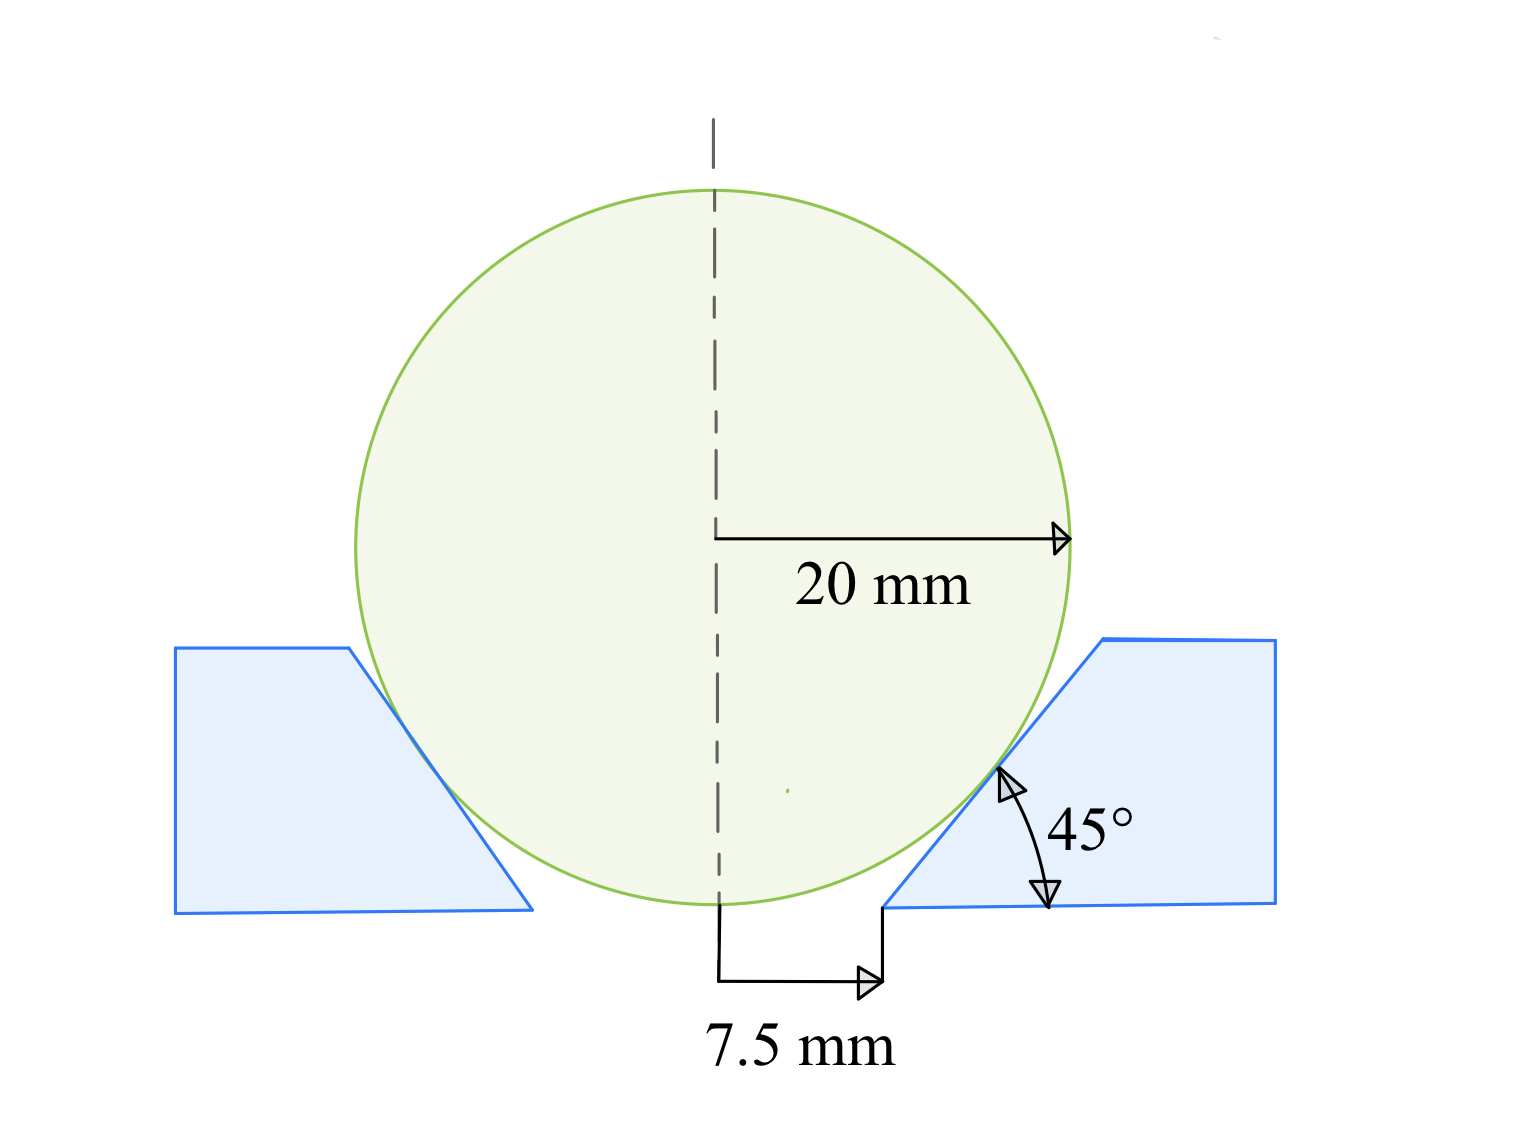
\includegraphics[width=0.3\textwidth]{figures/BallSeatValve/ballseatvalve.jpg}
    \caption{Sketch of ball seat valve.}
    \label{fig:ballseatvalve}
\end{figure}

%%%%%%%%%%%%%%%%%%%%%%%%%%%%%%%%%%%%%%%%%%%%%%%%%%%%%%%%%%%%%%%%%%%%%%%%%%%%%%
                      %%Sealing and leakage%%
%%%%%%%%%%%%%%%%%%%%%%%%%%%%%%%%%%%%%%%%%%%%%%%%%%%%%%%%%%%%%%%%%%%%%%%%%%%%%%%
\section{Sealing and Leakage}
\label{Sealing and Leakage}
The sealing performance of a valve is the ability of the valve's sealing component to prevent the leakage 
of medium. In order to control the flow of the fluids through a pipeline, valves must be installed, and 
the pipeline must be sealed to prevent leakage of the fluids it conveys. In the industrial manufacturing 
process, leaks from valves can have a detrimental influence on economic costs, safety, and environment, 
and can lead to significant production accidents; therefore, valves must have reliable sealing performance 
and meet the operating conditions' requirements 
for leakage. Therefore, it is necessary to investigate the sealing performance and leakage of valves.\\

In theory, the sealing principle of a ball seat valve is that the ball and the seat, both having 
perfectly smooth surfaces, are pressed against each other under load, and the two contact surfaces are 
entirely bonded together to prevent the passage of fluid from the valve in the pipeline, thereby achieving
a seal. In fact, however, it is not possible to obtain a theoretically smooth surface with 
modern machining technology.\cite{Sealing1} Consequently, it is common knowledge that there is no perfectly sealed valve in the world 
and that fluid leakage is bound to occur when the ball and seat are not fully bonded.\\

The sealing of a ball seat valve is determined by a large range of different factors.\cite{fischer2021influence}
For example, it is influenced by the roughness of the contact surfaces. Metallic surfaces are rough 
on a microscopic level.It must have uneven grooves and convex peaks. Due to the surface roughness, two rough 
planes which are apparently at full contact have a reduced real contact area if they 
are investigated using a higher resolution.\cite{fischer2021geometry} This means that when two 
rough sealing surfaces come into contact with each other,
 their highest peaks meet and microscopic channels are formed between the valleys, resulting in a leak.\\

 The sealing is also influenced by the applied forces and pressures on the system. When the load is increased,
  the two convex peaks in contact will be elastoplastically deformed to effectively increase the real contact area, 
  thereby reducing the size of the microscopic channel. However, the space between 
 the two corresponding valleys cannot be entirely eliminated, therefore a perfect seal is not achieved.\cite{Sealing2}
 In addition, the sealing is also influenced by temperature, the viscosity of the fluid in the pipe, etc. 
 In summary, the most important influencing factors that affect leakage can be divided into two main 
 categories: mechanical and hydraulic. Mechanical factors include those that act directly on the sealing 
 position through the valve. In contrast, hydraulic factors are introduced into 
 the system by the fluid. The Table \Ref{tab:influencing factors to valve} provides an overview of the most 
 important influential factors. \cite{PhD-M.S}


    \begin{table}[h!]
        \centering
        \begin{tabular}{||c| c |c |c||} 
         \hline
         Mechanical influencing factor & Hydraulic influencing factors  \\ [0.5ex] 
         \hline\hline
         Contact pressure  & Pressure difference  \\ 
         Macroscopic contact geometry & Temperature  \\
         Microscopic contact geometry & Viscosity \\
         Material hardness & Pollution \\
         Various material influences & Additive influences \\
         Geometric tolerance & Pressure pulsations\\[1ex] 
         \hline
        \end{tabular}
        \caption{The most important influencing factors to valve leakage.\cite{PhD-M.S}}
        \label{tab:influencing factors to valve}
        \end{table}

        It is impractical to discuss all the influencing factors simultaneously to analyze 
        the leakage of the ball seat valve. By controlling variables, the purpose of this study
         is to investigate the effect of the type and the 
        concentration of particles contained in the fluid on the leakage of the ball seat valve.